\documentclass[12pt]{article}
\usepackage{ctex}
\usepackage[T1]{fontenc}
\usepackage[utf8]{inputenc}
\usepackage{lmodern}
% textcomp package and marvosym package for additional characters
\usepackage{textcomp,marvosym}
\usepackage{lastpage}
\usepackage[tmargin=1cm,lmargin=2cm]{geometry}
% amsmath and amssymb packages, useful for mathematical formulas and symbols
\usepackage{amsmath, amssymb}
% cite package, to clean up citations in the main text. Do not remove.
\usepackage{cite}
% graphs
\usepackage{graphicx}
% outlines
\usepackage{titletoc}
\usepackage{ctexcap}
\usepackage{tikz}
\usepackage{pgfplots}
\pgfplotsset{compat=newest}
\usepackage{hyperref}
\linespread{1.5}
%
%
%
\begin{document}
%%%%%%%%
% first page
%%%%%%%%
\begin{figure}[h!]
\begin{minipage}[b]{\textwidth}
\centering

\includegraphics[scale=1.5]{./logo.png}
\end{minipage}
\begin{minipage}[b][30em]{\textwidth}
\centering
\Huge{Python程序设计} \vspace{1.5cm}\\
\huge{2022-2023-1} \vspace{1.5cm}\\
题目(题号): xxxxxxx\\
姓名(学号): xxxxxxxxx\\
班级: xxxxxxxx\\
\end{minipage}
\end{figure}
\date{}
\setcounter{page}{0}
\thispagestyle{empty}
% new page
\newpage

%%%%%%%%%
% outlines
%%%%%%%%%
\begin{center}
\titlecontents{section}
[4em]
{\bf \large}
{\contentslabel{2em}}
{}
{\titlerule*[1em]{$\cdot$}\contentspage}

\tableofcontents
\end{center}

\setcounter{page}{0} % main body starts from 1
\thispagestyle{empty}
% new page
\newpage

%%%%%%%%%
% Main Body
%%%%%%%%%%
\normalsize
%% title
\begin{center}
{\Large
\textbf\newline{项目名xxxxxxx} 
\
}
\newline  
%% insert author here
\\
姓名\textsuperscript{1*},
姓名\textsuperscript{2},
姓名\textsuperscript{3}
\\
\bigskip
\textbf{1} Leader, describe the main job
\\
\textbf{2} Team member, describe the main job
\\
\textbf{3} Team member, describe the main job 
\\
\bigskip
%
\end{center}

%% abstract
\begin{abstract}

This is the abstract about the paper, use at most 350 words to describe what the project is and what you have achieved.

\end{abstract}


%% section 1
\section{引言}

This is the first Section.

Some regular text and some symbols.

if you have some references ~\cite{ref1}, use the $cite$ command and refer to the number, like ~\cite{ref2}
 
\subsection{数学公式}
Here shows some math equations.

\begin{equation}
2*3 = 9
\end{equation}

\subsection{表格}

If you need to add some table, use it like this.

\begin{table}[!ht]
\centering
\caption{\bf{This is a table.}}
\begin{tabular}{rc|cl}
\hline
1&2&3&4\\
\cline{1
-
2}
&&&\\
4&5&6&7\\
\end{tabular}
\end{table}

\subsection{绘图}
\begin{figure}[ht!]
\centering
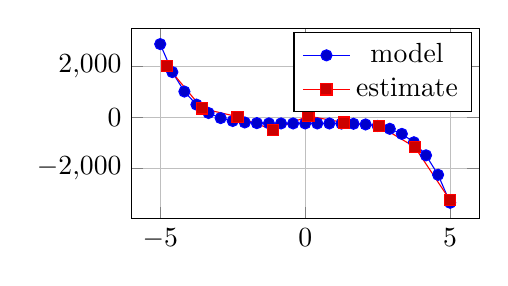
\begin{tikzpicture}
\begin{axis}[height=4cm, width=6cm, grid=major]
\addplot{-x^5 - 242};
\addlegendentry{model}
\addplot coordinates {
(-4.77778,2027.60977)
(-3.55556,347.84069)
(-2.33333,22.58953)
(-1.11111,-493.50066)
(0.11111,46.66082)
(1.33333,-205.56286)
(2.55556,-341.40638)
(3.77778,-1169.2478)
(5.0,-3269.56775)
};
\addlegendentry{estimate}
\end{axis}
\end{tikzpicture}
\caption{\bf{This is the plot.}}
\end{figure}

%%%%%
\subsection{图格式}
\begin{figure}[ht!]
\centering
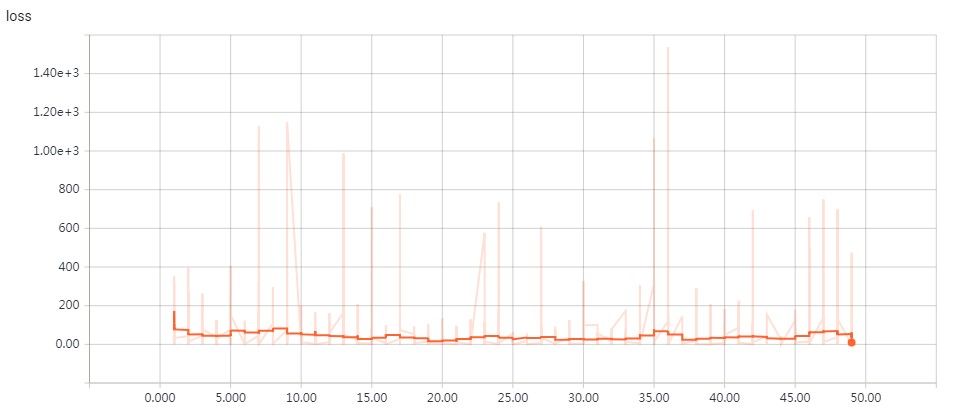
\includegraphics[scale=0.5]{./loss.jpg}
\caption{\bf{This is the result.}}
\end{figure}



%%   Section 2
\section{系统设计}
\subsection{概要设计}
\subsubsection{系统框架设计}
\subsubsection{系统功能设计}
\subsection{功能设计}
\subsubsection{功能1}
\subsubsection{功能2}
\subsection{数据库设计}



%%  Section 3
\section{系统实现}
\subsection{前端实现}
\subsection{后端实现}

%%  Section  4
\section{结束语}
\subsection{总结}
\subsection{不足与展望}


%% reference
\begin{thebibliography}{10}

\bibitem{ref1}
Gunarathne T, Wu T-L, Choi JY, Bae S-H, Qiu J.
\newblock Cloud computing paradigms for pleasingly parallel biomedical applications.
\newblock Concurrency and Computation-Practice \& Experience. 2011;23(17):2338-54.

\bibitem{ref2}
Kiviluoto K.
\newblock Topology preservation in self-organizing maps.
\newblock IEEE International Conference on Neural Networks. 1996.

\end{thebibliography}


%
\end{document}